\documentclass[11pt,a4paper]{article}
\usepackage[margin=2.5cm]{geometry}
\usepackage{amsmath,amssymb,amsthm,mathtools,bm}
\usepackage{graphicx,booktabs,enumitem,xcolor,tabularx}
\usepackage{tikz}
\usetikzlibrary{positioning,arrows.meta,shapes.geometric}
\usepackage[colorlinks=true,linkcolor=blue!50!black,urlcolor=blue!50!black]{hyperref}
\usepackage{microtype}
\graphicspath{{figures/data_quality/}}

\theoremstyle{definition}
\newtheorem{definition}{Definition}
\theoremstyle{remark}
\newtheorem*{remark}{Remark}
\newcommand{\R}{\mathbb{R}}
\newcommand{\1}{\mathbf{1}}
\newcommand{\code}[1]{\texttt{\detokenize{#1}}}
\newcommand{\Nb}{\mathcal{N}_8}

\title{How the data-quality assessment of the OPERA archive was computed}
\author{Notes for the \texttt{minkowski-loss} project}
\date{23 September 2026}

\begin{document}
\maketitle

\begin{abstract}
These notes describe the data-quality audit run on 23 September 2026 over the raw OPERA
radar archive: 745 days, 4.8 million tiles of $128\times128$ pixels. They cover every step
from the stored rain rate to the summary tables:
\begin{itemize}[nosep]
\item what is read;
\item how tiles are cut and keyed;
\item how a per-pixel clutter climatology is built;
\item the exact definition of each of the $\sim$45 per-tile features;
\item the candidate artefact rules;
\item the statistics in the summary;
\item the split-leakage audit;
\item the image gallery used for labelling.
\end{itemize}
Each quantity is defined mathematically and illustrated. A final part reports the first
full-run results and how the code was checked.

The audit \emph{describes} the data. It deletes nothing, and its rule thresholds are
starting guesses to be calibrated against labels.
\end{abstract}

\tableofcontents

%======================================================================
\section{What the assessment is for}
%======================================================================

The project's claims are about the upper tail of rain rate. Artefacts of the radar network
concentrate in that tail: ground and sea clutter, interference spokes, range rings, one-frame
bursts and decoding errors. A patch ranked by its maximum is therefore more likely to be an
artefact the higher it ranks. The audit answers four questions before any screening
decision is made:
\begin{enumerate}[nosep]
\item Which artefact \emph{signatures} are present, and how common are they as a function of
  intensity, year, season, time of day and location?
\item Which ones overlap, so that a single rule would suffice, and which ones are
  independent?
\item What does the current preprocessing (\code{filter_precip_bounds}) do to the tail?
\item How independent are the current train/validation/test splits?
\end{enumerate}
Everything is computed on the \emph{raw} stored field, before any filtering, and on the full
downloaded archive, not only on the patches that entered training.

%======================================================================
\section{The data it reads}
%======================================================================

\paragraph{Grid and time.}
Each day is one zarr store \code{RAW_OPERA_DATA_DIR/YYYYMMDD/}. It holds a rain-rate array
$R_t(y,x)$ in mm/h, for $t$ over the day's 15-minute composites and $(y,x)$ on the OPERA
2\,km Lambert azimuthal equal-area grid of $2200\times1900$ pixels. Pixels outside radar
coverage are \code{NaN}, and ``no echo'' is $0$. Stores written by the archive fetcher
(\code{scripts/data/fetch_opera_archive.py}) also carry the OPERA total quality index
$Q_t(y,x)\in[0,1]$. Figure~\ref{fig:domain} shows the coverage.

\begin{figure}[t]
\centering
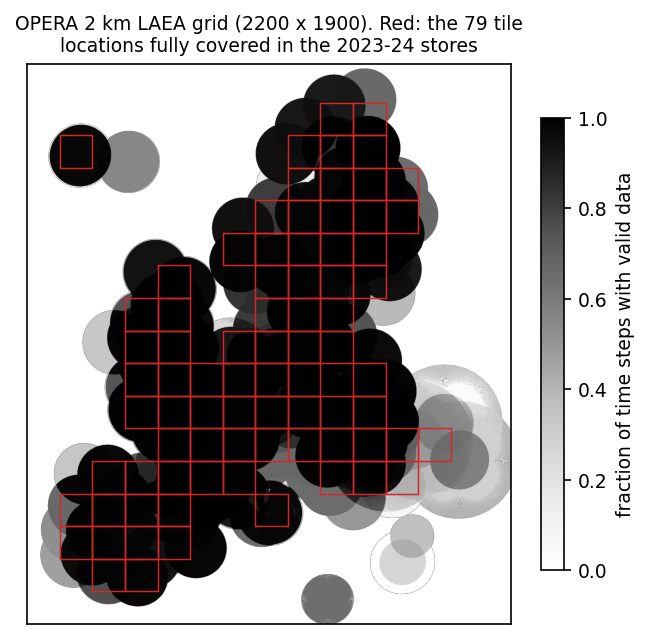
\includegraphics[width=0.55\linewidth]{fig_domain.png}
\caption{Fraction of time steps with valid data at each pixel over all 745 days (grey), and
the tile locations that are fully covered in the 2023--24 stores (red). Tiles are
$128\times128$ pixels ($256\times256$\,km) on a stride-128 grid.}
\label{fig:domain}
\end{figure}

\paragraph{Two kinds of store.}
The raw directory mixes two sources, and they differ in a way that matters.
\begin{itemize}[nosep]
\item \textbf{Original 2023--24 stores} (Aug 2023 -- Oct 2024, 442 days): the source of the
  current patch set. They hold the rate only, no QIND.
\item \textbf{Fetched archive stores} (2012--13 and test days in 2016, 2020 and July 2023,
  303 days): written by the fetcher. They hold rate and QIND, with no alteration of values.
\end{itemize}
Figure~\ref{fig:range} compares their tile maxima. The original stores \emph{never exceed
150\,mm/h}. Over their 2,853,816 fully covered tiles the maximum is exactly $150.0$ and the
99.99th percentile is $149.94$. The archive stores continue smoothly past 150 and reach
$\sim10^5$\,mm/h (decoding errors and clutter).
\begin{itemize}[nosep]
\item So the 150\,mm/h cut is present in the original raw source itself, not only in our
  preprocessing. Whether the source clipped or removed the values above 150 cannot be told
  from the stores.
\item Recovering real 2023--24 peaks would need those days re-fetched from the archive.
\end{itemize}

\begin{figure}[t]
\centering
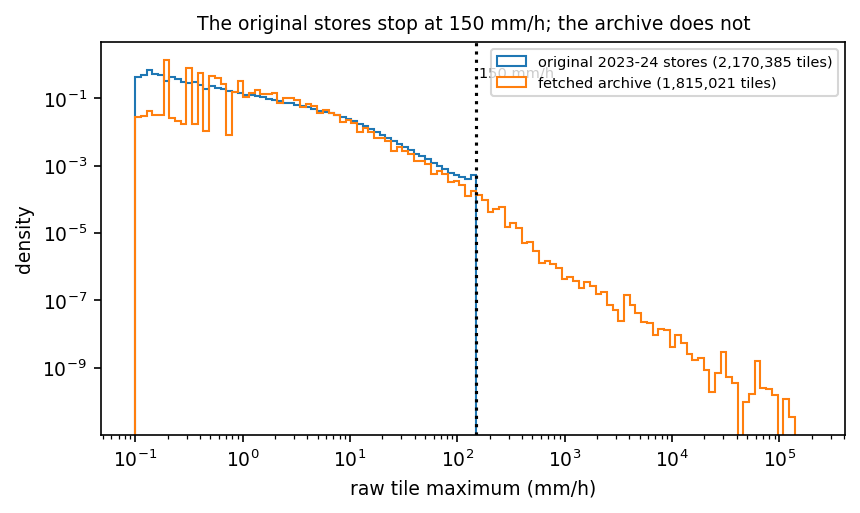
\includegraphics[width=0.72\linewidth]{fig_value_range.png}
\caption{Distribution of raw tile maxima in the two kinds of store (tiles with max $>0.1$\,mm/h).}
\label{fig:range}
\end{figure}

%======================================================================
\section{Pipeline overview}
%======================================================================

\begin{figure}[h]
\centering
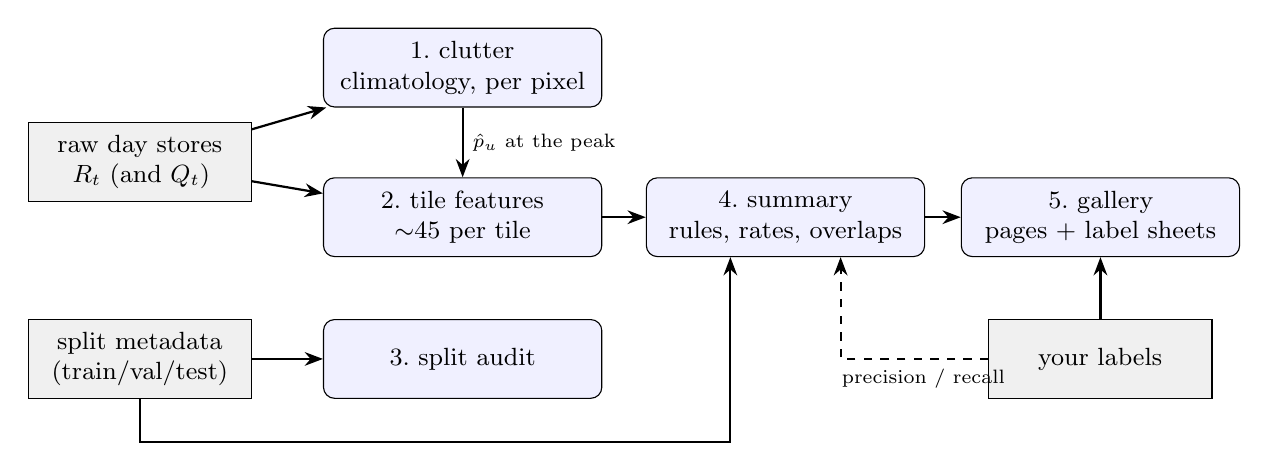
\begin{tikzpicture}[every node/.style={font=\small},
  box/.style={draw,rounded corners,align=center,fill=blue!6,minimum height=10mm,text width=33mm},
  dat/.style={draw,align=center,fill=gray!12,minimum height=10mm,text width=26mm},
  arr/.style={->,>=Stealth,thick}]
\node[dat] (raw)   at (0,  0.9) {raw day stores\\ $R_t$ (and $Q_t$)};
\node[dat] (meta)  at (0, -1.6) {split metadata\\ (train/val/test)};
\node[box] (clim)  at (4.1, 2.1) {1.\ clutter\\ climatology, per pixel};
\node[box] (feat)  at (4.1, 0.2) {2.\ tile features\\ $\sim$45 per tile};
\node[box] (split) at (4.1,-1.6) {3.\ split audit};
\node[box] (sum)   at (8.2, 0.2) {4.\ summary\\ rules, rates, overlaps};
\node[box] (gal)   at (12.2, 0.2) {5.\ gallery\\ pages + label sheets};
\node[dat] (lab)   at (12.2,-1.6) {your labels};
\draw[arr] (raw) -- (clim);
\draw[arr] (raw) -- (feat);
\draw[arr] (clim) -- node[right]{\scriptsize $\hat p_u$ at the peak} (feat);
\draw[arr] (meta) -- (split);
\draw[arr] (feat) -- (sum);
\draw[arr] (meta.south) -- ++(0,-0.55) -| ([xshift=-7mm]sum.south);
\draw[arr] (sum) -- (gal);
\draw[arr] (lab) -- (gal);
\draw[arr,dashed] (lab.west) -| node[pos=0.22,below]{\scriptsize precision / recall} ([xshift=7mm]sum.south);
\end{tikzpicture}
\caption{The five stages of \code{scripts/hpc/launch_data_quality.sh}. Dashed: the labelling
loop, which closes after you label tiles.}
\label{fig:pipeline}
\end{figure}

Stage by stage (all scripts are in \code{scripts/data_quality/}; the feature definitions are
in \code{src/data/quality.py}):
\begin{enumerate}[nosep]
\item \code{clutter_climatology.py} counts, per pixel, how often each threshold is exceeded
  (\S\ref{sec:clim}).
\item \code{compute_tile_features.py} cuts every tile at every time step and computes the
  features (\S\ref{sec:features}). Clutter frequencies from stage 1 are joined at the tile's
  peak.
\item \code{audit_splits.py} measures the overlap of the current splits (\S\ref{sec:splits}).
\item \code{summarize_features.py} applies the candidate rules and aggregates
  (\S\ref{sec:rules}--\ref{sec:summary}).
\item \code{patch_gallery.py} renders tiles for inspection and writes label sheets
  (\S\ref{sec:gallery}).
\end{enumerate}

%======================================================================
\section{Tiles and keys}
%======================================================================

A tile is identified by its time stamp $t$ and its lower-left pixel $(r,c)$, with $r,c$
multiples of 128. It is the array
\begin{equation}
  T(i,j) = R_t(r+i,\;c+j),\qquad 0\le i,j<128 .
\end{equation}
The tile grid, the key format \code{timestamp,row,col} and the orientation are exactly those
of \code{scripts/preprocess/generate_metadata.py}. So every feature row joins one-to-one onto
the existing patch metadata. A tile is kept when its coverage
$\mathrm{cov}(T)=\frac1{128^2}\sum_{ij}\1[T(i,j)\ \text{finite}]$ equals 1 (flag
\code{--min_coverage}), which is the current patch definition.

\begin{remark}[Alignment check]
Applying the pipeline's own filter to a tile and taking the maximum reproduces the
\code{max_precip} column of the metadata exactly (difference $0.0$ on every joined test
tile). The number of fully covered tiles in the original stores, 2,853,816, equals the total
number of train + validation + test patches. Both checks confirm that the audit sees exactly
the tiles the model was trained on.
\end{remark}

%======================================================================
\section{Stage 1: the clutter climatology}\label{sec:clim}
%======================================================================

A real storm crosses a given pixel a handful of times a year. Ground clutter, wind farms,
sea clutter and interference light up the \emph{same} pixels again and again. For every pixel
and threshold $u\in\{1,31,89,150,500\}$\,mm/h, over all time steps of all days:
\begin{align}
  n(y,x)   &= \sum_t \1\big[R_t(y,x)\ \text{finite}\big], \\
  n_u(y,x) &= \sum_t \1\big[R_t(y,x)\ge u\big], \qquad
  \hat p_u(y,x) = \frac{n_u(y,x)}{\max(n(y,x),1)} .
\end{align}
The estimate $\hat p_u$ is the empirical exceedance frequency. Weather varies smoothly in
space on these scales, while clutter is pixel-sharp. The \emph{local excess}
\begin{equation}
  e_u(y,x)=\hat p_u(y,x)-\operatorname{med}_{15\times15}\hat p_u(y,x)
\end{equation}
therefore removes the climatological background (a $15\times15$ median filter, 30\,km) and
keeps what stands out from its surroundings. The script also stores yearly counts, the
per-pixel maximum and the mean QIND, and it ranks the top-$50$ pixels by $e_{31}$
(\code{clutter_hotspots.csv}). Figure~\ref{fig:clim} shows the result: sharp spokes
radiating from individual radars, complete range rings, and a fan of interference.

\begin{figure}[t]
\centering
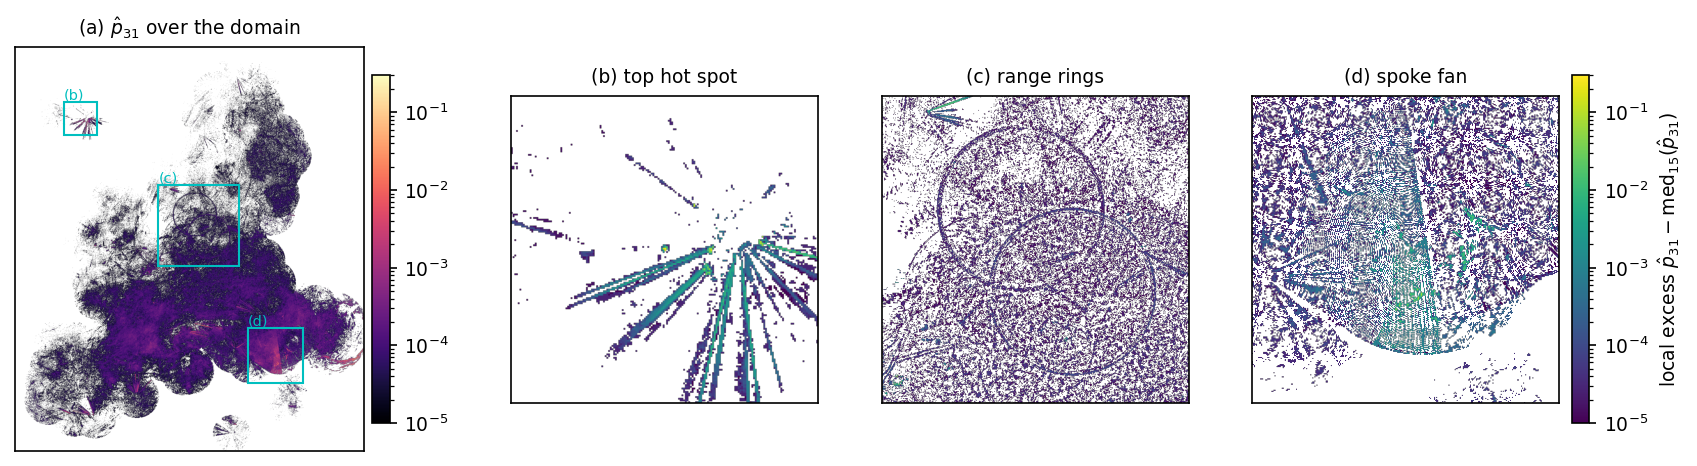
\includegraphics[width=\linewidth]{fig_climatology.png}
\caption{(a) Exceedance frequency of 31\,mm/h over all 745 days. (b--d) Local excess $e_{31}$
in three zooms. The top hot-spot pixel exceeds 31\,mm/h in 23\% of all time steps.}
\label{fig:clim}
\end{figure}

The tile features join two numbers from this map (\S\ref{sec:featclim}):
$\hat p_u$ at the tile's peak pixel, and the maximum of $\hat p_u$ over the tile.

%======================================================================
\section{Stage 2: the tile features}\label{sec:features}
%======================================================================

All features are computed on the raw tile $T$, with $\mathrm{NaN}$ treated as missing. The
notation used throughout:
\begin{itemize}[nosep]
\item $Z=T$ with $\mathrm{NaN}\to0$;
\item $M=\max Z$, the tile maximum, attained at $p^\star=(i^\star,j^\star)$;
\item $\Nb(p)$, the eight neighbours of pixel $p$ (edge pixels have fewer);
\item $\delta=0.1$\,mm/h, the drizzle level;
\item $D=150$\,mm/h, the current declutter threshold.
\end{itemize}
Figure~\ref{fig:sig} applies the actual feature code to synthetic tiles that isolate one
signature each.

\begin{figure}[t]
\centering
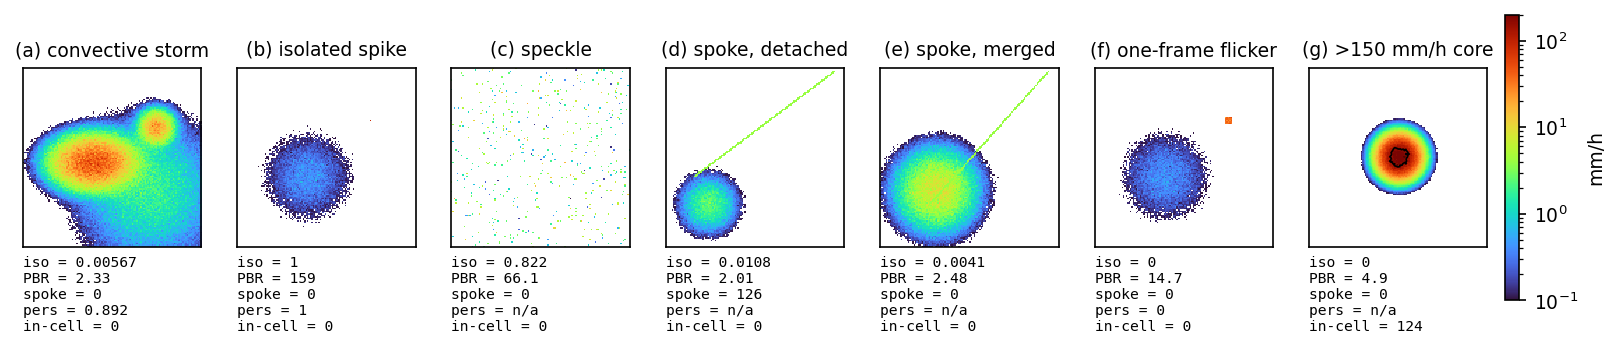
\includegraphics[width=\linewidth]{fig_signatures.png}
\caption{Synthetic tiles and the values the audit computes for them. \code{iso}: isolated
fraction at 1\,mm/h. \code{PBR}: peak/coarse-block ratio. \code{spoke}: spoke length in px.
\code{pers}: persistence into $t-15$. \code{in-cell}: pixels $>150$\,mm/h inside a cell.
Panel (e) shows a known limitation: a spoke that touches rain merges with it and is not
detected.}
\label{fig:sig}
\end{figure}

\subsection{Intensity and concentration}
\begin{align}
  M&=\max_{ij}Z_{ij},\qquad \bar T=\operatorname{mean}_{\text{finite}}T,\qquad
  q_{99}=\text{99th percentile},\\
  \mathrm{wet}&=\tfrac1{|T|}\#\{T\ge\delta\},\qquad
  N_u=\#\{T\ge u\}\ \ (u\in\{1,31,53,89,150,500\}),\\
  \mathrm{conc}&=\bar T/M .
\end{align}
The \emph{concentration} is near 0 when the tile's rain is carried by a few pixels. A real
convective cell raises $M$ and the wet area together, so conc falls only slowly with $M$.
A single bright pixel drives it to $\sim10^{-4}$.

\subsection{Speckle, spikes and gradients}
Let $\mathrm{nbmax}(p)=\max_{q\in\Nb(p)}Z_q$, with $\mathrm{nbmean}$, $\mathrm{nbmed}$ and
$\mathrm{nbmin}$ defined likewise.
\begin{itemize}
\item \textbf{Isolated fraction} at level $u\in\{0.1,1,10\}$: the share of pixels
  $\ge u$ with no neighbour $\ge u$,
  \begin{equation}
    \mathrm{iso}_u=\frac{\#\{p:\ Z_p\ge u,\ \mathrm{nbmax}(p)<u\}}{\#\{p:\ Z_p\ge u\}} .
  \end{equation}
  Rain fields are spatially coherent at 2\,km, so $\mathrm{iso}_u$ is small for weather and
  large for speckle (Fig.~\ref{fig:sig}c: $0.82$).
\item \textbf{Spikes}: pixels $\ge10$\,mm/h whose brightest neighbour is below a quarter of
  them, $\mathcal S=\{p: Z_p\ge10,\ \mathrm{nbmax}(p)<\tfrac14Z_p\}$. The features are
  $n_{\text{spikes}}=|\mathcal S|$ and the \emph{spike mass fraction}
  $\sum_{\mathcal S}Z/\sum Z$.
\item \textbf{Peak-to-neighbour ratio}: $\;M/(\mathrm{nbmean}(p^\star)+\delta)$.
\item \textbf{Maximum gradient}: the largest absolute difference between 4-neighbours,
  $\max|T_{i+1,j}-T_{ij}|\vee|T_{i,j+1}-T_{ij}|$, in mm/h per 2\,km.
\end{itemize}

\subsection{Connected components and the spoke detector}
Components are the 8-connected sets of $\{Z\ge u\}$ for $u\in\{1,31\}$. The features are the
number of components and the size of the largest.

Interference spokes are long, thin and straight. For each component $C$ with $|C|\ge30$ px,
take the covariance of its pixel coordinates,
\begin{equation}
  \Sigma_C=\frac1{|C|}\sum_{p\in C}(p-\bar p)(p-\bar p)^\top,\qquad
  \lambda_{\max}\ge\lambda_{\min}\ \text{its eigenvalues}.
\end{equation}
The \emph{elongation} $\epsilon_C=1-\sqrt{\lambda_{\min}/\lambda_{\max}}$ is $0$ for a disc
and tends to $1$ for a line. A uniform segment of length $L$ has variance $L^2/12$ along its
axis, so
\begin{equation}
  L_C=\sqrt{12\,\lambda_{\max}}
\end{equation}
estimates the component's length. The features are $\max_C\epsilon_C$ and the
\emph{spoke length} $\max\{L_C:\epsilon_C>0.9\}$ (Fig.~\ref{fig:sig}d: $126$\,px).

\begin{remark}
A spoke crossing a rain area is part of a larger, non-elongated component and is invisible
to this detector (Fig.~\ref{fig:sig}e). Detecting it would need radar-site geometry (azimuth
from the site), which the audit does not have.
\end{remark}

\subsection{Relation to the coarse input}
The model is conditioned on a $10\times10$ coarse field made by
\code{torch.nn.functional.adaptive_avg_pool2d} of the \emph{filtered} tile. With $n=128$ and
$m=10$, bin $k$ covers pixels
\begin{equation}
  \big[\lfloor kn/m\rfloor,\ \lceil (k+1)n/m\rceil\big),
\end{equation}
which are 13 or 14 pixels wide and overlap by one (Fig.~\ref{fig:pool}). The audit
reproduces these bins exactly (unit-tested against torch). Let $\bar B(p^\star)$ be the mean
of the coarse block containing the peak. Then
\begin{equation}
  \mathrm{PBR}=\frac{M}{\bar B(p^\star)+\delta}.
\end{equation}
A lone pixel in an otherwise dry block gives $\mathrm{PBR}\approx$ the block area ($\sim170$).
A convective core, whose surroundings are also wet, gives single digits. A large PBR means
the target contains a peak that the input gives no hint of, which is exactly what makes
artefacts harmful to a super-resolution model.

\begin{figure}[t]
\centering
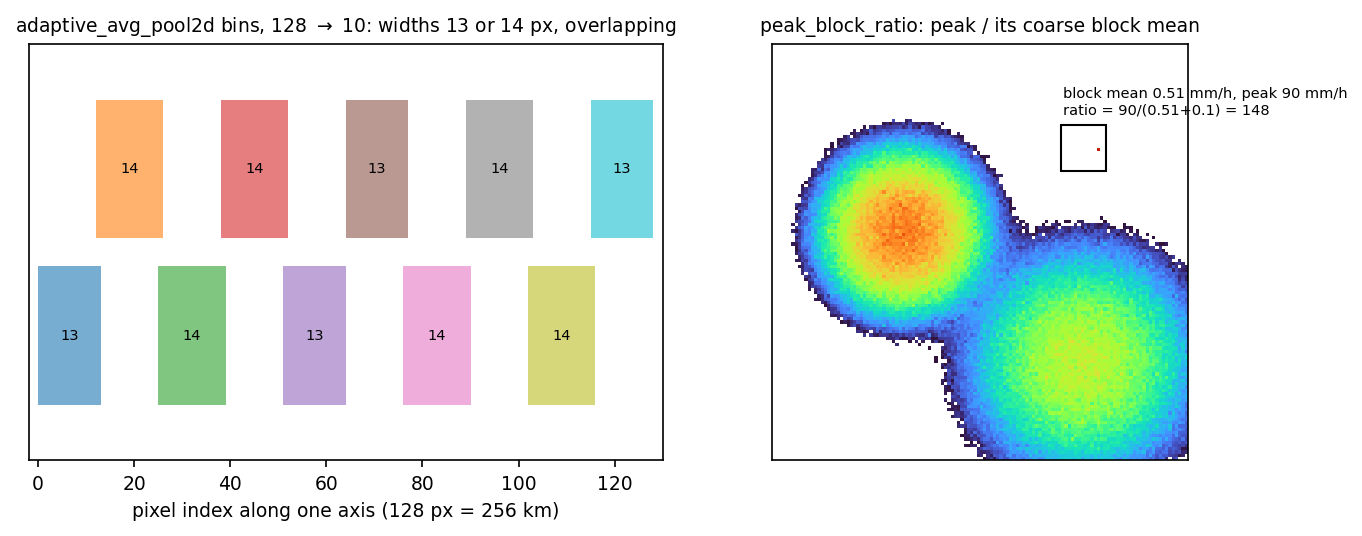
\includegraphics[width=0.85\linewidth]{fig_pooling.png}
\caption{Left: the ten adaptive-pooling bins along one axis. Right: the peak/coarse-block
ratio for an isolated 90\,mm/h pixel.}
\label{fig:pool}
\end{figure}

\subsection{What the current declutter step does}
\code{filter_precip_bounds} sets every value outside $[\delta,D]$ to zero, and
\code{NaN} to zero. The audit counts
\begin{equation}
  n_{>D}=\#\{p: Z_p>D\},\qquad
  n_{>D}^{\text{cell}}=\#\{p: Z_p>D,\ \mathrm{nbmed}(p)\ge10\},
\end{equation}
the second being the pixels above 150 that sit \emph{inside} a wet area. Zeroing those
punches a hole in the storm (Fig.~\ref{fig:hole}, top). It also counts pre-existing holes,
$\#\{p: Z_p<\delta,\ \mathrm{nbmin}(p)\ge10\}$.

\begin{figure}[t]
\centering
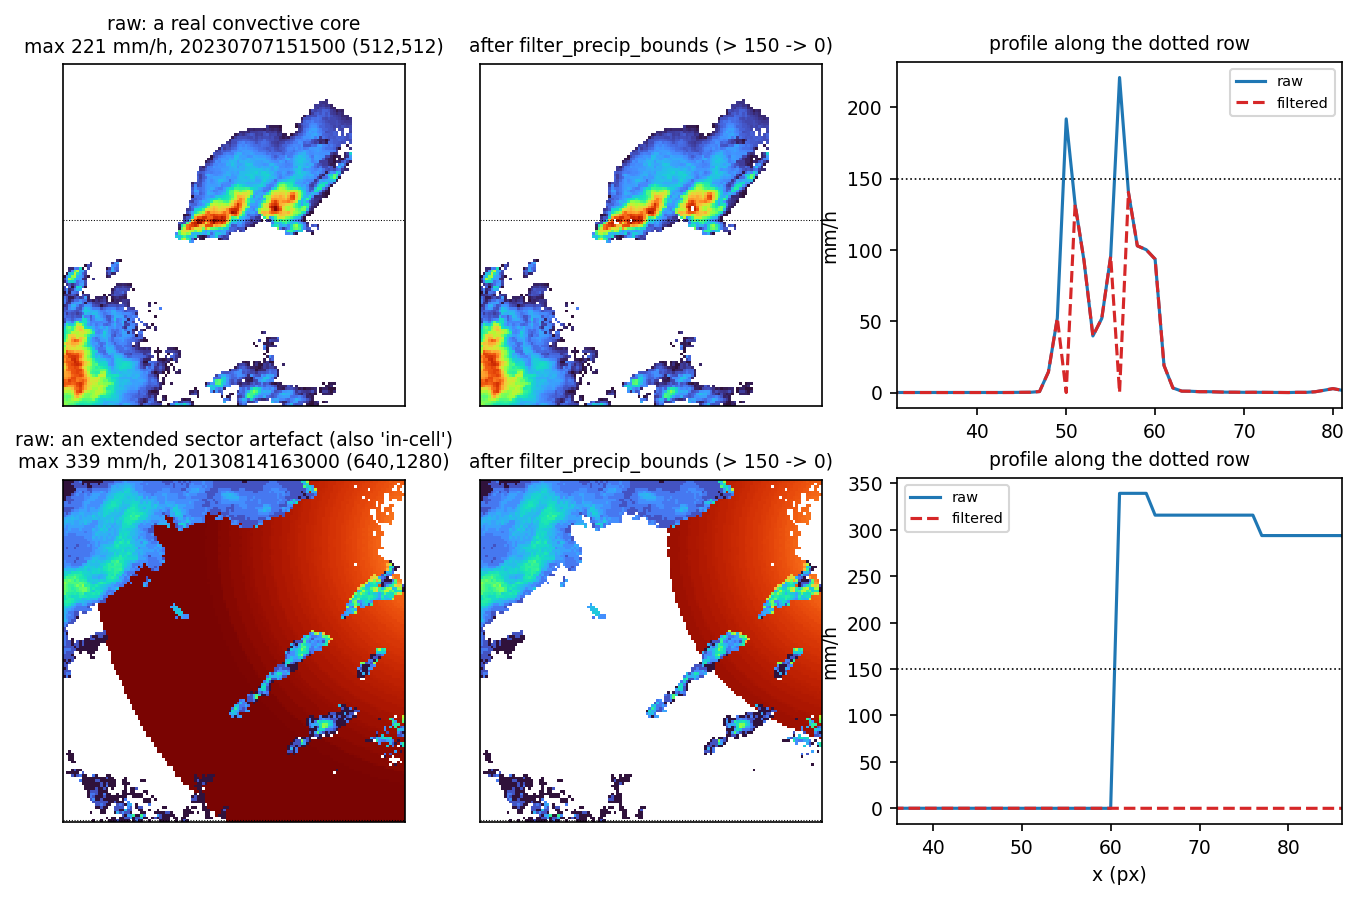
\includegraphics[width=0.93\linewidth]{fig_hole.png}
\caption{Top: a real convective core from the fetched July 2023 data. Its two peaks above
150\,mm/h are set to 0 by the current filter, leaving holes at the storm's centre. Bottom:
an extended high-value sector artefact. It also passes the ``inside a cell'' test, because
its neighbours are high too. The in-cell count therefore identifies holes in real storms only
together with the other features.}
\label{fig:hole}
\end{figure}

\subsection{Terrain and sea}
With the DEM on the same grid, sea is $\{\mathrm{DEM}\le0\}\cup\{\mathrm{DEM}\ \text{missing}\}$.
The features are:
\begin{itemize}[nosep]
\item the sea fraction and mean elevation;
\item whether the peak lies over sea;
\item the share of wet ($\ge1$\,mm/h) pixels that lie over sea.
\end{itemize}
Sea clutter shows up as intense peaks over sea in coarse blocks that are almost dry.

\subsection{OPERA's quality index}
Where the store has QIND:
\begin{itemize}[nosep]
\item its coverage $\#\{Q\ \text{finite}\}/\#\{T\ \text{finite}\}$;
\item the mean of $Q$ over all pixels, over wet pixels and over pixels $\ge31$\,mm/h;
\item the share of $\ge31$\,mm/h pixels with $Q<0.5$;
\item $Q(p^\star)$.
\end{itemize}
The QIND coverage is itself informative: in the archive it is missing on most of the covered
area.

\subsection{Persistence in time}
Real storms persist and move. At 15-minute resolution a cell moving at $\le50$\,km/h
travels $\le12.5$\,km, about 6 pixels. With $W$ the $13\times13$ window centred on $p^\star$
($\pm6$\,px), and $R_{t\pm1}$ the neighbouring frames of the same tile:
\begin{equation}
  \mathrm{pers}_{\pm}=\frac{\max_{W}R_{t\pm1}}{M}.
\end{equation}
A persistent storm gives values near 1: the median for tail tiles with a large core in 2024
is $0.88$. A one-frame burst gives $\approx0$ in both directions (Fig.~\ref{fig:sig}f).

Values well above 1 are also informative: the neighbouring frame holds something much
brighter nearby, typically a burst in \emph{that} frame. The Pearson correlation of
$\log(1+R_t)$ with $\log(1+R_{t-1})$ over the tile is recorded as \code{corr_prev}. The first
and last frames of a day have no neighbour across the day boundary, and their persistence is
missing.

\subsection{Static clutter at the peak}\label{sec:featclim}
From stage 1: $\hat p_u(p^\star)$ at the tile's peak pixel, and $\max_T\hat p_u$ over the
tile, for each $u$. A tile peaking on a pixel that exceeds 31\,mm/h in more than 1\% of all
time steps is almost certainly peaking on clutter.

A caveat: this is only as good as the climatology. On a few days it flags recurring
\emph{weather} too. Over 745 days it isolates the static artefacts.

%======================================================================
\section{Stage 4a: candidate rules}\label{sec:rules}
%======================================================================

Each rule turns features into a flag for one signature. \textbf{The thresholds are first
guesses}, to be calibrated against labels (\S\ref{sec:gallery}).

\begin{center}\small
\begin{tabularx}{\linewidth}{@{}lX@{}}
\toprule
rule & flag condition \\ \midrule
spike & $n_{\text{spikes}}>0$ and spike mass fraction $>0.2$ \\
speckle & $\mathrm{iso}_1>0.5$ and $N_1<200$ \\
isolated\_peak & $M\ge10$ and $\mathrm{PBR}>60$ \\
flicker & $M\ge10$ and $\max(\mathrm{pers}_-,\mathrm{pers}_+)<0.2$ \\
sea\_clutter & $M\ge10$, peak over sea, and $\bar B(p^\star)<0.5$ \\
spoke & spoke length $>40$\,px (80\,km) \\
static\_clutter & $M\ge31$ and $\hat p_{31}(p^\star)>0.01$ \\
qind\_low & $M\ge10$ and $Q(p^\star)<0.3$ \\
declutter\_isolated & $n_{>D}>n_{>D}^{\text{cell}}$ (pixels $>150$ outside any wet area) \\
unphysical & $M>500$\,mm/h \\
\midrule
declutter\_hole & $n_{>D}^{\text{cell}}>0$: not an artefact flag; the tiles the current filter would hole \\
\bottomrule
\end{tabularx}
\end{center}

\paragraph{Missing inputs are not ``no''.}
A rule whose inputs are missing gives $\mathrm{NaN}$, not $0$. Examples are
\code{qind_low} on stores without QIND, and \code{flicker} at the first frame of a day. Rates
are then computed over tiles where the rule is defined. \code{any_flag} is 1 if any defined
rule fires, and missing only if no rule is defined.

%======================================================================
\section{Stage 4b: the summary statistics}\label{sec:summary}
%======================================================================

\paragraph{Strata.}
Tiles are grouped by raw maximum $M$ into $[0,0.1)$, $[0.1,1)$, $[1,10)$, $[10,31)$,
$[31,53)$, $[53,89)$, $[89,150)$, $[150,500)$ and $[500,\infty)$\,mm/h. The \emph{tail} is
$M\ge31$\,mm/h, the POT level of the project's tail protocol. Stratifying by the raw maximum
defines the tail before anything is removed.

\paragraph{Flag rates.}
For a group $G$ and rule $k$, $\hat\pi_k(G)=\frac1{|G_k|}\sum_{G_k}f_k$ over the tiles
$G_k\subseteq G$ where $f_k$ is defined. The binomial standard error
$\sqrt{\hat\pi(1-\hat\pi)/|G_k|}$ understates the true uncertainty: tiles of the same storm
and the same hour are strongly correlated. Treat differences below a few percentage points
as noise until they are recomputed with day-level resampling.

\paragraph{The key diagnostic.}
In a clean archive, artefact signatures would become \emph{rarer} towards the tail, because
real extremes are large coherent storms. A flag rate that rises with $M$ is therefore
evidence of contamination, whatever the rules' individual precision.

\paragraph{Overlap.}
Rules $k,l$ are compared by the Jaccard index over the tail,
$J_{kl}=|F_k\cap F_l|/|F_k\cup F_l|$, where $F_k$ is the set of flagged tiles. Small off-diagonal
values mean the rules catch different things, so a screen needs their union.

\paragraph{Breakdowns and outputs.}
Rates are also broken down by year, month, hour (UTC), current split and tile location. The
summary lists every flagged tail tile (\code{flagged_tail.csv}, 216,714 tiles) for the
gallery.

\paragraph{Against labels.}
Given a sheet of labelled tiles (artefact / real / unsure), each rule gets
\begin{equation}
  \text{precision}=\frac{TP}{TP+FP},\qquad \text{recall}=\frac{TP}{TP+FN}
\end{equation}
over tiles labelled artefact or real. Labels must come from a \emph{random} draw of the tail
as well as from flagged tiles. Otherwise precision cannot be separated from the base rate.

%======================================================================
\section{Stage 3: the split audit}\label{sec:splits}
%======================================================================

\code{split_metadata.py} shuffles individual patches, so the same storm can be in train and
test. For each test (and validation) patch $(t,r,c)$ the audit asks whether the train split
contains:
\begin{itemize}[nosep]
\item \emph{same time}: any patch at the same $t$;
\item \emph{same tile within 1\,h}: a patch at $(t',r,c)$ with $|t'-t|\le60$\,min (found by
  binary search in the tile's sorted train times);
\item \emph{adjacent tile, same time}: a patch at $(t,r\pm128,c\pm128)$.
\end{itemize}

\begin{center}\small
\begin{tabular}{@{}llrrrr@{}}
\toprule
query & subset & $n$ & same time & same tile $\pm$1\,h & adjacent, same $t$ \\ \midrule
test & all & 285,383 & 100.0\% & 100.0\% & 98.2\% \\
test & patch max $\ge31$ & 25,591 & 100.0\% & 100.0\% & 99.4\% \\
test & patch max $\ge89$ & 6,349 & 100.0\% & 100.0\% & 99.3\% \\ \bottomrule
\end{tabular}
\end{center}
Validation gives the same numbers. Every current test score is therefore an interpolation
score within storms seen in training.

%======================================================================
\section{Stage 5: the gallery and the labelling loop}\label{sec:gallery}
%======================================================================

\code{patch_gallery.py} renders one row per tile (Fig.~\ref{fig:gallery}):
\begin{itemize}[nosep]
\item the raw frames at $t-15$, $t$ and $t+15$ min;
\item the target after the current filter, where holes show as white;
\item the coarse input as the model sees it;
\item the DEM and QIND.
\end{itemize}
The row header carries the key, the raw maximum and the rules that fire. The selections are:
\begin{itemize}[nosep]
\item \code{top_max}: the highest maxima;
\item \code{rule:<name>}: the tiles each rule flags;
\item \code{unflagged}: tail tiles no rule flags, to find misses;
\item \code{random}: an unbiased draw from the tail, needed for precision and recall.
\end{itemize}
Each page set comes with \code{labels.csv}. Fill its \code{label} column and pass the file to
\code{summarize_features.py --labels} to close the loop in Fig.~\ref{fig:pipeline}.

\begin{figure}[p]
\centering
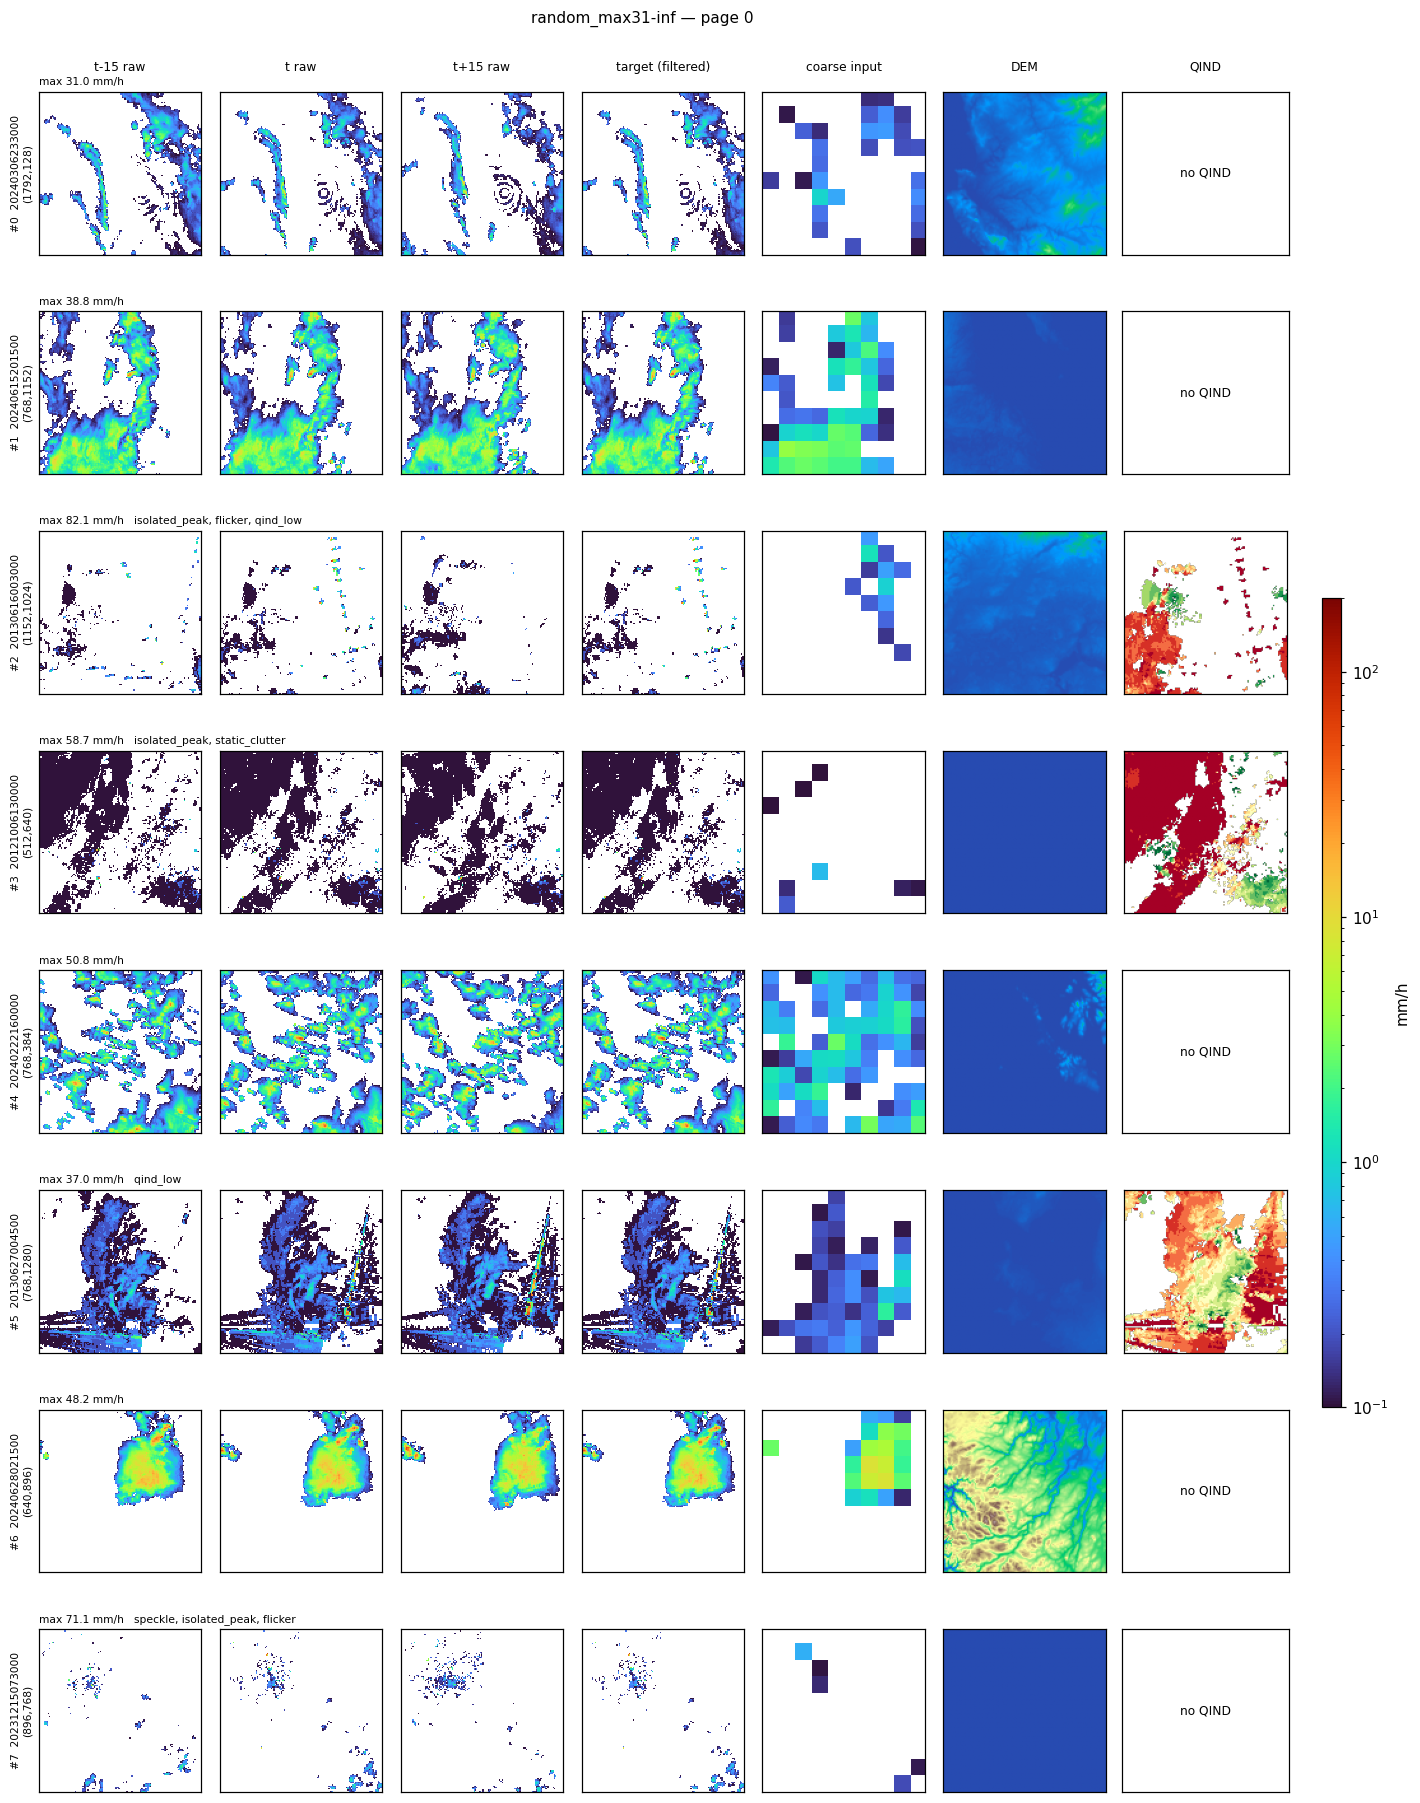
\includegraphics[width=0.92\linewidth]{fig_gallery_random.png}
\caption{First page of the random tail draw. Rows 1, 4 and 6 are real storms with no rule
firing. Rows 2, 3 and 7 are flagged artefacts. Row 0 is a real storm with a ring artefact
that no rule catches. Row 5 is a storm crossed by a spoke that merges with the rain. Only
\code{qind_low} fires there; the spoke rule misses it (Fig.~\ref{fig:sig}e).}
\label{fig:gallery}
\end{figure}

%======================================================================
\section{First full run: what it shows}
%======================================================================

The full run took about 4 hours with 6 workers on 8 cores. It covered 745 days (2012-09-04 to
2024-10-30) and 4,804,051 tiles, of which 413,654 (8.61\%) are in the tail.

\begin{figure}[t]
\centering
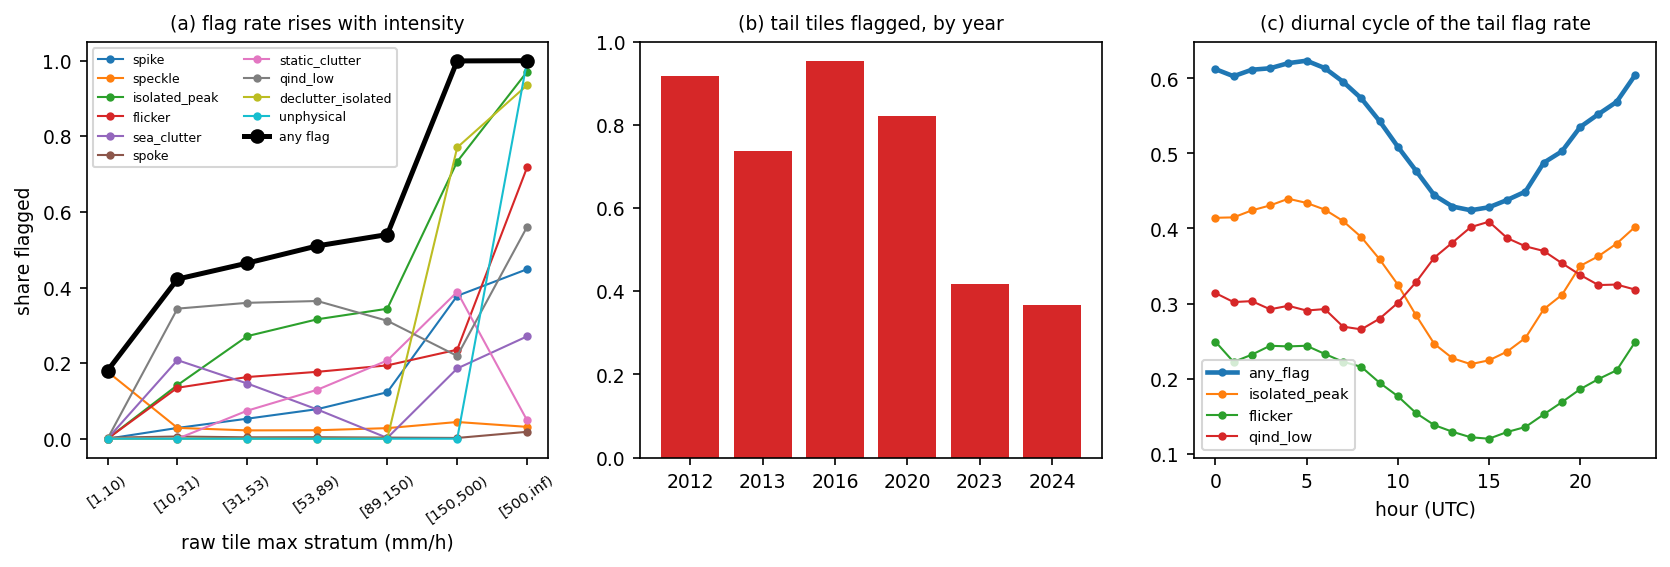
\includegraphics[width=\linewidth]{fig_rates.png}
\caption{(a) Flag rate by raw-max stratum, per rule and for any rule. (b) Share of tail tiles
flagged, by year. (c) Diurnal cycle of the tail flag rate.}
\label{fig:rates}
\end{figure}

\begin{enumerate}
\item \textbf{The flag rate rises with intensity} (Fig.~\ref{fig:rates}a). Any-flag is
  18\% of tiles at 1--10\,mm/h, 47\% at 31--53, 54\% at 89--150, and $\approx100\%$ above
  150. That is the contamination signature of \S\ref{sec:summary}.
\item \textbf{Old years are dirtier} (Fig.~\ref{fig:rates}b). 92\% of 2012 tail tiles are
  flagged, 75\% in 2013, and 42\% and 37\% in 2023 and 2024. The QIND-based rule exists only
  for the fetched years.
\item \textbf{A diurnal cycle} (Fig.~\ref{fig:rates}c). The tail flag rate is $\approx61\%$ at
  night and $\approx43\%$ mid-afternoon. Two effects combine: nighttime clutter (anomalous
  propagation under stable layers) and afternoon convection adding real tail tiles.
\item \textbf{The rules are complementary.} Most tail Jaccard indices are below 0.3; the
  largest is \code{isolated_peak} with \code{flicker} (0.36). No single rule is a screen.
\item \textbf{Static clutter is real and located} (Fig.~\ref{fig:clim}). A few tile
  locations have 85--97\% of their tail tiles flagged. The worst is (1024, 640).
\item \textbf{The declutter step touches 5.7\% of tail tiles.} It would hole real cells in
  7,867 of them, all in the fetched years, since the original stores stop at 150.
\end{enumerate}

\begin{figure}[t]
\centering
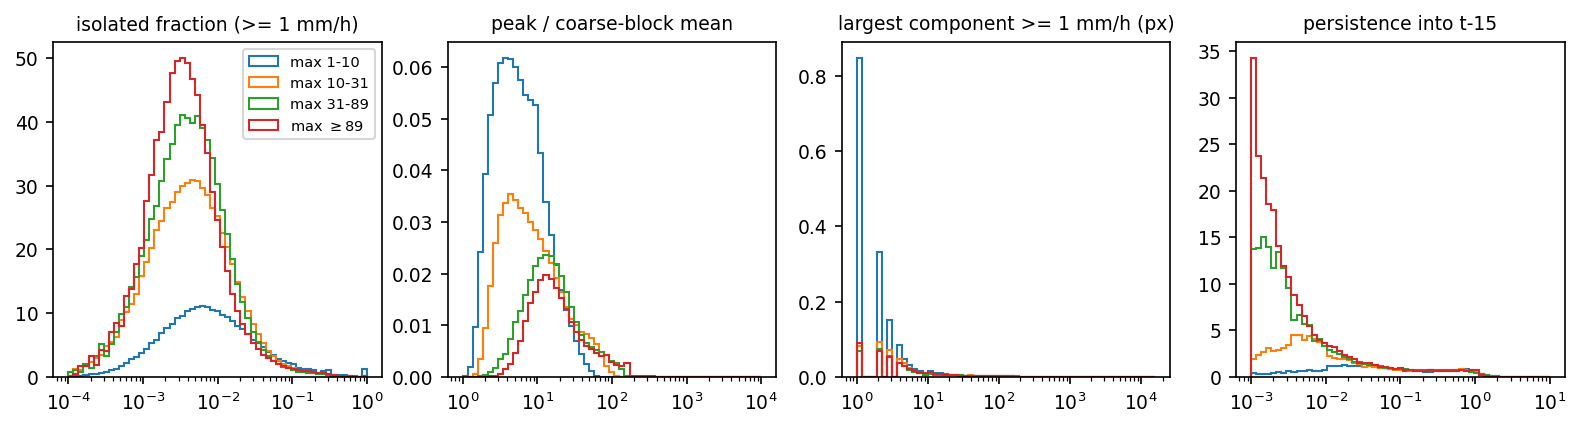
\includegraphics[width=\linewidth]{fig_features.png}
\caption{Four features by raw-max stratum (tiles with max $\ge1$\,mm/h; log-spaced bins,
density per bin). Persistence has a long low tail (the flicker cases, $\approx10\%$ of the
tail). Log-spaced bins plotted as density visually exaggerate that tail. The median
persistence is 0.53--0.72 in every stratum.}
\label{fig:features}
\end{figure}

%======================================================================
\section{How the code was checked}
%======================================================================

\begin{itemize}
\item \textbf{Unit tests} (\code{tests/test_quality.py}, 8 tests). Each artefact feature must
  separate its synthetic artefact from a synthetic storm: spike against storm, the spoke's
  length within 5\%, flicker against advection, and declutter-in-cell against isolated. The
  coarse pooling is checked against \code{adaptive_avg_pool2d} to $10^{-6}$, and NaN and
  all-NaN tiles are handled.
\item \textbf{Alignment.} The filtered tile maximum reproduces the metadata \code{max_precip}
  exactly. The original-store tile count equals the patch count.
\item \textbf{Smoke tests} on 5 days before the full run, with visual inspection of the
  gallery pages.
\item \textbf{Sanity checks on the full run.}
  \begin{itemize}[nosep]
  \item The distributions behave as expected by stratum (Fig.~\ref{fig:features}).
  \item The persistence of large real cores has a median of 0.88.
  \item Extreme persistence ratios ($>10^3$, 65 tiles) trace to bursts in the neighbouring
    frame, not to arithmetic errors.
  \end{itemize}
\end{itemize}

%======================================================================
\section{Limitations}
%======================================================================
\begin{itemize}[nosep]
\item Rule thresholds are uncalibrated. The rates measure signature prevalence, not artefact
  counts.
\item There is no radar-site geometry, so spokes and rings merged with rain are missed
  (Fig.~\ref{fig:sig}e, Fig.~\ref{fig:gallery}, rows 0 and 5).
\item The in-cell criterion for $>150$\,mm/h pixels is fooled by extended artefacts
  (Fig.~\ref{fig:hole}, bottom).
\item Flag rates are correlated across tiles of the same storm, so the standard errors are
  optimistic.
\item QIND exists only in the fetched stores, and even there it is missing on much of the
  domain.
\item Tiles with partial coverage are excluded, following the current patch definition. The
  domain edge is therefore under-represented.
\end{itemize}

%======================================================================
\section*{Reproducing}
%======================================================================
\begin{verbatim}
# whole audit, CPU only, cores 4-11 (see EXPERIMENTS.md §0)
setsid bash scripts/hpc/launch_data_quality.sh \
    /home/fquareng/work/data/extremes/OPERA/quality 6 &
# after labelling:
python scripts/data_quality/summarize_features.py config.yaml \
    --features_dir .../quality/features --out_dir .../quality/summary \
    --labels .../quality/gallery/random_max31-inf/labels.csv
# figures in these notes:
python notes/figures/make_data_quality_figures.py
\end{verbatim}

\end{document}
